% !TeX root = rbenford.tex
\title{Modeling of disaster death tolls with Benford’s Law }
\author{by Abdullah Al Mahmud}

\maketitle

\abstract{
In 1938, physicist Frank Benford showed that among many naturally occurring collections of numbers, the leading significant digit is expected to be small, a pattern which was first indicated by astronomer Simon Newcomb and is now known as Benford's law or Newcomb-Benford's law. According to the law, in a set where the law fits, most numbers begin with digit 1, accounting for over 30\% of total numbers, and the frequency of numbers starting with later digits falls almost exponentially. This law has been shown to apply to multitude of natural data sets, including stock and house prices, population numbers, death rates, length of large objects, and mathematical constants, among others. In this paper, we have tested the conformity of the law (for the first significant digit) with the number of deaths due to four different disasters: earthquakes, wars, accidents, and floods, and found significant agreement with the law, a result which can be applied to analyze, model, cross-check, and predict various disaster death tolls. The compliance was tested with Pearson's Chi-squared goodness-of-fit test as well with some other testing procedures specific to the law, including Leemis’s m statistic. In the process, we have developed an efficient R ~ \citep{R} function to automate the testing procedure. 
}

\section{Introduction}
The Benford’s law deals with the first significant digits of numbers. For example, the first significant digits of the numbers 976 and 167 are 9 and 1, respectively. Since a number can start with digits 1, 2, … up to 9, it is natural to assume that the probability of any of the nine numbers being the first digits of a randomly chosen number is $\frac{1}{9}$. However, in many real world data sets, it is seen that the frequencies of numbers starting with each digit (1-9) are in strong congruence with what is predicted by Benford’s law ~ \citep{benf}. That is, the smaller digits are seen to appear most as the leading significant digit of a number, 1 appearing over 30\% of time, 2 appearing 17.5 \% of time, 3 appearing 12.5 \% of time, and so on and so forth. The anomalous theoretical frequencies according to the law are shown in Table ~\ref{exp_freq}. 

The law, though popularized by Frank Benford, traces its back to an 1881 work by the mathematician and astronomer Simon Newcomb, who showed that ten digits in the logarithmic table do not occur with equal frequency ~\citep{Newcomb:1996}.  He concluded that numbers in logarithmic tables obey the pattern, while anti-logarithms do not ~ \citep{steven}. He then proposed a law that the probability of a single number N being the first digit of a number would be equal to  $\log({N+1})-\log({N})$.   

The law generated a great number of papers, dealing with matters including theoretical developments, verifying the law for numbers of bases other than 10 (decimal numbers), explanation of the pattern ~ \citep{fewster}, testing compliance with real-world data, scale invariance ~\citep{roger}, applications to various phenomena  ~ \citep{diek}, including for legal and accounting purposes, price digit analysis ~\citep{morrow}, detection of fraudulent scientific data ~\citep{seh}, as well as developing of statistical tests to verify agreement with the law such as by ~\citet{leemis} and ~ \citet{cho}. 

In his paper, Benford (1937) demonstrated several data sets to comply with the law, including surface areas of 335 rivers, 3259 US populations, 104 physical constants, 1389 specific heat values, 703 pressure data, 1165 Black Body data, and 418 death rates, among others ~ \citep{kvam}. It was later shown by ~\citet{theo} that data sets containing uniformly numbers of several orders of magnitude (e.g. populations) agree with the Benford’s law, while data sets with numbers with mainly within only one order of magnitude (e.g. IQ scores) mostly, if not always, defy the law. Many well-known integer sequences have been shown to comply with the law, among them being Fibonacci numbers ~\citep{washt}, the powers of 2 ~\citep{raimi}, and continuous growth processes, especially exponential growth or decay mechanism. 

Empirical tests were carried out ~\citep{formann} to test the compliance of several important probability distributions with the Benford's law, among them being the uniform distribution, the the exponential distribution, the half-normal distribution, the right-truncated normal, the normal distribution, the chi square distribution and the log normal distribution. It was found that while the uniform distribution iteself does not obey the law, the ratio distribution of two uniform distributions complies well with the law. Several benchmark testing procedures have been suggested to test for agreement with the Benford’s law. Pearson’s chi-squared test is the de facto test in this scenario, while Kolmogorovo-Smirnov and Kuiper tests are better for small sample sizes ~\citep{steph}.  There are some tests which are specific to the law, like the test statistics proposed by~\citet{leemis} and ~\citet{cho}. 

The purpose of this paper is to test the compliance of the number of deaths due to disaster with the Benford’s law, carrying out the relevant statistical tests, and to reexamine, to greater extent, the compliance of the law with populations of countries (testing for 263 countries and territories, both with small and large populations). The findings can be applied to detecting fraudulent data, disaster-related policy-making, as well to estimate the expected number of death tolls due to disasters.  

\subsection{Mathematics of Benford’s law}
A collection of numbers is said to obey the Benford’s law if the first digit d (where d $\epsilon \{1,...,9\}$ ) has the probability of occurring 
\begin{equation} 
\begin{split}
P(d) &= \log{_{10}(d+1) - \log{_{10}(d)}} = \log{_{10}(\frac{d+1}{d})} = \log{_{10}(1+\frac{1}{d})}
\end{split}
\end{equation}

Where, P (d) is the percentage of numbers starting with the digit d.  
The distribution of the leading digits according to the law is shown in Table ~\ref{exp_freq}. The law can be stated for bases other than 10 as well for second and later significant digits. For any number system with base b, the law can be stated as follows: \\
\begin{equation} 
\begin{split}
P(d) &= \log{_{b}(d+1) - \log{_{b}(d)}} = \log{_{b}(\frac{d+1}{d})} = \log{_{b}(1+\frac{1}{d})}
\end{split}
\end{equation}

Also, since the law can be generalized to digits other than the first, the probability that d (d=0,1,…,9) is found as the nth digit is 
\begin{equation} 
\sum_{k=10^{n-2}}^{10^{n-1}-1} \log{_{10}(1+\frac{1}{10k+d})} \\
\end{equation}
For example, the probability that digit 2 is placed as the second digit is \\
\begin{equation} 
\begin{split}
\log{_{10}(1+\frac{1}{12})}+\log{_{10}(1+\frac{1}{22})}+...+\log{_{10}(1+\frac{1}{92})} = 0.109 (approximately)
\end {split}
\end{equation}

\begin{table}
\begin{center}
\caption{Frequencies of digits according to Benford's law}
\label{exp_freq}
\begin{tabular}{|c| c |c| c| c| c| c| c| c| c|} 
\hline

Digit&1&2&3&4&5&6&7&8&9\\
\hline

Percentage&30.1 &17.5&12.5&9.7&7.9&6.7&5.8&5.1&5.6\\
\hline
\end{tabular}
\end{center}
\end{table}

\section{Data and Methodology}

\subsection{Data collection and processing  }
The primary variable in the study is number of deaths due four disasters: earthquakes, flood, accidents, and wars. For all the types of disasters, the data were collected from all over the world, focusing primarily on the deadliest cases on record with respect to number of deaths. The data on earthquakes were collected from various relevant sources, among them being the Unites States Geological Survey (USGS), International Association of Engineering Geology, National Geophysical Data Center etc.; on accidents from various news sources including ~\citet{BBC:hope}, Global Active Archive of Large Flood Events ~\citep{Brakenridge}, ~\citet{Age}, and Brisbane Times etc.; on wars from 
~\citet{nash}, ~\citet{Age}, among others, and on flood from Global Active Archive of Large Flood Events, ~\citet{Worldometers}, and the Dawn etc. Whenever an interval of estimate was found instead of a single number, the lowest estimate was considered. Among the types of accidents considered were structural fires and collapses, road, aviation and maritime accidents, explosions, industrial disasters, and sporting events. Additionally, gathered were data of populations of 263 countries and dependencies since 1960 until 2016, totaling 57 years of data for 263 regions ~\citet{seh}. The entire analysis was performed using R programming language ~\citep{R}, including the \CRANpkg{tidyverse} package ~\citep{tidyverse}. 

\subsection{Test procedure}
Since the obtained frequencies in our analysis are not small (all the frequencies are greater than five), the chi-squared test of goodness-of-fit, a test procedure for checking observed frequencies with expected frequencies, can be assumed to be perfect to test for the compliance with the law. The relevant test statistic is as follows: \\
\begin{equation}
\chi^2=\sum_{i=1}^n {\frac{(O_i-E_i)^2}{E_i}} = N\sum_{i=1}^n \frac{(\frac{O_i}{N}-p_i)^2}{p_i}
\end{equation}

Where, $\chi^2$ = Pearson's cumulative test statistic, which asymptotically approaches a $\chi^2$ distribution.\newline
$O_i$ = the number of observations of type i.\newline
$E_i$ = the expected number of count of type i, as stated by the null hypothesis that the proportion of type i in the population is $p_i$. \newline
and n = number of cells in the table. \\

For the chi-squared test statistic, the null hypothesis is that there is no difference between observed and expected frequencies of numbers. If p-values obtained from the estimation are greater than 0.01 and 0.05, for instance, this will imply that the observed frequencies are in compliance with the expected frequencies (as predicted by Benford’s law) at 0.01 and 0.05 levels of significance, respectively. Although the chi squared test can be used to test for compliance with Benford's law, the statistical power of the test is low when the sample size is small. Two better alternative tests for small sample are Kolmogorov–Smirnov test and the Kuiper test. Since the samples we are dealing with are quite large for carrying out statistical tests, we are not currently interested in these tests. 

Tests which are specific to this law are also available due to ~\citet{leemis} and ~\citet{cho}. 
The test statistic proposed by Leemis et al is known as max (m) or Lemis’s m and defined as below: \\

\begin{equation}
m={\sqrt {N}}\cdot \operatorname {*} \max _{i=1}^{9}{\Big \{}|\Pr(X{\text{ has FSD}}=i)-\log _{10}(1+1/i)|{\Big \}}
\end{equation}

Where FSD is the first significant digit and N is the sample size. 
And the test statistic, called the distance statistic (d) or Cho-Gaines’d, proposed by Cho et, al is as follows: \\

\begin{equation}
d={\sqrt {N\cdot \sum _{i=1}^{9}{\Big [}\Pr(X{\text{ has FSD}}=i)-\log _{10}(1+1/i){\Big ]}^{2}}}
\end{equation}


\begin{table}
\begin{center}
\caption{Critical regions of Leemis’s m and Cho-Gaines’s test statistics at different levels of statistical significance}
\label{cr}
\begin{tabular}{c|ccc}
$\alpha $ & 0.10 & 0.05 & 0.01 \\
\hline
\text{Leemis’ m} & 0.851 & 0.967 & 1.212 \\
\text{Cho-Gaines’ d} & 1.212 & 1.330 & 1.569 \\
\end{tabular}
\end{center}
\end{table}

In table ~ \ref {cr}, $\alpha$ is the level of significance of the test, and if the observed value of the test statistics is less than the values on the table, then it is decided that the data do obey the Benford’s law in given level of significance. 

\subsection{ \code {rben} \textbf{function}}
Our goal is to count the number of data points beginning with each of the nine digits (1 to 9). The function starts working by eliminating the negative sign, if any, followed by converting the numbers to characters, in order to make use of the \code {strsplit} function. The \code {strsplit} function provides a list of isolated characters, from which the first characters are extracted. Then the characters, which are just the first digits of each number, are converted back to numerical values. Thus, it now remaines to just count the frequencies of each digit. In order to create an organized dataframe from the output, the dplyr package was used. The function creates graphs using the expected and empirical perceteanges of numbers for each of the nine digits. Additionally, the results of chi-squared test as well as m and d statistics, proposed by ~\citet{leemis} and ~\citet{cho}, respectively, were also generated. The properties of function are shown in Figure ~ \ref{rben}.\\

\begin{figure}[htbp]
 \caption{\code {rben} \textbf{function}}
  \label{rben}
\begin{tabular}{ll}
\hline
\code {rben}&  \text{Testing compliance with Benford's law} \\
\hline
\text{\textbf{Description}} & \text{} \\
\text{} & \text{This function test whether a data complies with Benford's law.} \\
\text{\textbf{Usage}} & \text{} \\
\text{} & \text{\code{rben}(x, TRUE, title)} \\
\text{\textbf{Arguments}} & \text{} \\
\text{x} & \text{A numeric vector} \\
\text{plot} & \text{logical; if TRUE, the results will be shown on a graph} \\
\text{title} & \text{Name of data} \\
\text{\textbf{Details}} & \text{} \\
\text{}  & \text{A function to test compliance with Benford's law} \\
\text{\textbf{Example}} & \text{} \\
\text{} & \text{rben(1:100, "N")} \\
\hline
\end{tabular}
\end{figure}



\section{Results and discussion}
\subsection{Testing of disaster data}
The studied dataset contains a total of 193 severe floods from all over the world, spanning more than a millennium, while a total of 197 significant wars have been considered. Included are both World War I and II, Gallic wars, Crimean War, Crusades, Vietnam War, Napoleonic Wars, and so on. Also, 190 cases of floods and 1538 cases of different accidents from all over the world were used in the analysis. The result is shown in table ~ \ref{result} and the Figure ~  \ref{ben_res}.\\


\begin{table}
\caption{Summary of disaster death tolls with expected and observed frequencies of numbers starting with digits 1 through 9. }
\label{result}
\begin{tabular}{p{0.3in}p{0.7in}p{0.7in} p{0.7in}p{0.7in}p{0.7in}}
\hline
Digit & Expected percentage (by Benford’s Law, \%) & Observed percentage
(Floods, \%) & Observed percentage
(Earthquakes, \%) & Observed percentage
(Wars, \%) & Observed percentage
(Accidents, \%)\\
\hline
1&30.1&26.42&26.32&35.53&35.7\\
2&17.61&22.8&20.53&16.75&17.88\\
3&12.49&15.03&14.21&9.64&10.4\\
4&9.69&10.36&8.95&9.64&6.89\\
5&7.92&6.74&8.42&7.11&7.09\\
6&6.69&4.15&7.37&4.57&7.15\\
7&5.8&3.63&5.26&5.58&5.53\\
8&5.12&6.74&5.26&5.58&4.62\\
9&4.58&4.15&3.68&5.58&4.75\\
\hline
\end{tabular}
\end{table}

Figure ~ \ref{ben_res} as well as table 2 and 3 suggest a strong agreement of the four studied data sets with Benford’s law. While the percentages of the digit 1 for floods and earthquakes are 26.42 and 26.32, both being less than the corresponding expected frequencies, the percentages of wars and accidents data sets for the same digit (1) exceed what is stated by Benford’s law, being 35.53 and 35.7, respectively i.e. the first digit percentages exceed expected percentage by almost 5\%. All data sets, however, seem, from the graphical illustrations, to satisfy the law. This is confirmed by the p-values for all data sets except for accidents, the p-value being almost 0. For accidents data set, Pearson’s chi-squarest test as well as tests based on Leemis’ m and Cho-Gaines’ d differ from the graphical connotation. This contradiction might have resulted from the fact that although we have covered many different types of accidents, many other types remain to be explored. Still, the pattern of distribution of number to different digits conforms to Benford’s distribution. All other chi-squared p-values are well above 0.01, being no less than 0.28 and as high as 0.93, indicating clear and strong conformity with Benford’s law. Also, test results from Leemis’ m and Cho-Gaines’ d provide strong evidence in favor of conformity of floods, wars, and earthquakes death tolls with Benford’s law. 

The critical values for the Leemis' m are 0.851, 0.967, and 1.212 for the significance levels 0.10, 0.05, and 0.00, respectively. And, the observed values of the test statistic corresponding to floods, earthquakes, wars, and accidents data are 0.72, 0.52, 0.76, and 2.19, respectively. This suggests that all except for accidents data seem to defy the law, a result concerning which we have proposed an explanation. Similar argument holds for the Cho–Gaines' d statistic. 

\begin{figure}[htbp]
  \centering
  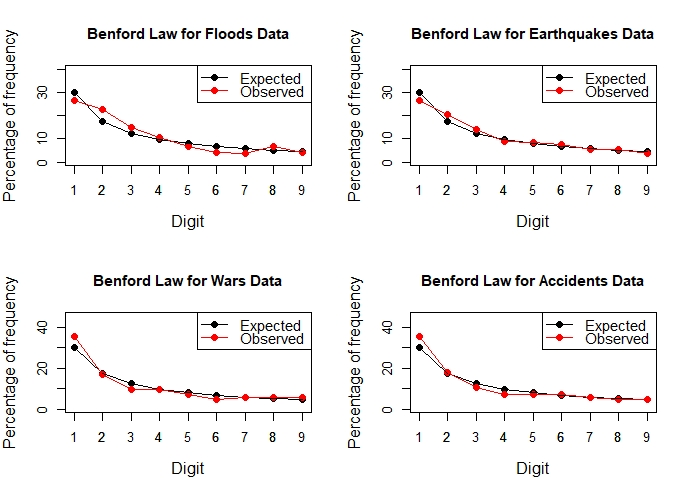
\includegraphics[width=0.70 \paperwidth]{ben_res}
  \caption{\textbf {Expected and empirical percentages and frequencies of numbers starting with digits one through nine for disaster death tolls.} The red points and lines represent the observed percentages of numbers with each significant digits, while the black points and lines represent the expected and observed percentages of frequencies of numbers, respectively.}
  \label{ben_res}
\end{figure}

Table ~ \ref{test_res} reveals that according to Leemis’ m, the floods, earthquakes, and wars data sets are in strong conformity with the Benford’s law, while accidents data set is not, exactly as was suggested by the chi-squared tests. Also, by Cho-Gaines’ d measure, all data sets except the accidents satisfy the law. The agreement of three different tests lead us to conclude that death tolls due to floods, earthquakes, as well wars can be modeled by Benford’s law, while accidents death tolls may not agree with the law for small sample size. 

Thus, the findings can be applied to detect artificial anomaly or fraud in data set related to disasters. Although, we have performed the analysis only for four types of disasters, it is expected that the law will hold for other disaster as well such as landslide, volcanic eruptions, tornadoes, cyclones, tsunamis etc. 

\subsection{Test with populations data}
For this large-scale re-examination procedure, the world populations comprising of 263 countries and territories were considered. Earlier, ~\citet{sandron} showed that populations of 198 countries or geopolitical entities as of the year 1997 followed Benford’s law. Here, we have performed the analysis with the data of 57 years: from 1960 to 2016, each year dealt separately, carrying out the above tests, and recording the associated p-values and other statistics. The resulting p-values are shown in Figure ~ \ref{ben_test_pop}. 

\begin{table}
\caption{Summary of statistical test of conformity }
\label{test_res}
\begin{tabular}{c|cccc}
\text{Data} & \text{Flood} & \text{Earthquake} & \text{Wars} & \text{Accidents}\\
\hline
\text{Pearson’s chi-squared test p-value} & 0.28 & 0.93 & 0.72 & \textless 0.001 \\
\text{Leemis’ m} & 0.72 & 0.52 & 0.76 & 2.19 \\
\text{Cho-Gaines’d} & 1.10 & 0.73 & 0.94 &  2.62 \\
\end{tabular}
\end{table}


Of the 57 years analyzed, no instance was found where the chi-squared test p-value was below 0.01, which implies world population data of different territories in any year conforming to Benford’s law, at 1\% level of statistical significance. Only three instances were found where p-values are only slightly greater than 0.1. It must be noted here that when we intend to comply with null hypothesis , as in the case that we are now dealing with, the evidence in greater level of significance is always stronger. Since all p-values except for three are well above 0.10, most being close to or above 0.5, this indicates a very strong compliance with the Benford's law.  The fact that the compliance is very strong is further justified from the finding that only one p-value is below 0.05 (in the case of the year 1960), which indicates that all other cases are very strongly congruent with Benford’s law.

Also examined were Leemis’ m and Cho-Gaines’ d measures. They have also been found to be uncompromising; at 1\% level of significance, in stark dovetail with chi-squared test, no case could be concluded to defy the law—neither by Leemis’ m nor by Cho-Gaines’  d statistics. Thus, strong compliance with the law has been established. Therefore, these findings can be applied to detect fraud or artificial anomaly in the figures related to populations of different territories at a given instant of time. 

\begin{figure}[h]
  \centering
  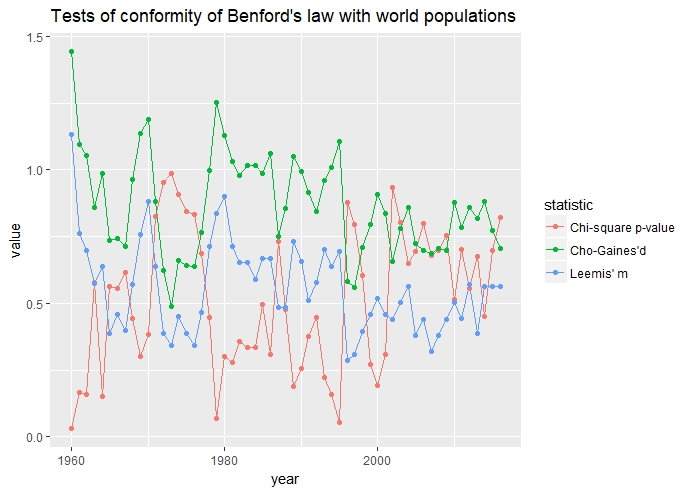
\includegraphics[width=\textwidth]{ben_test_pop}
  \caption{\textbf {Chi-squared p-values and observed values of Leemis’ m and Cho-Gaines’ d test statistics in testing whether yearly world populations of 263 countries and territories conform to Benford’s law, with each year dealt separately. A total of 57 years were analyzed.}}
  \label{ben_test_pop}
\end{figure}

The result can be applied as a criterion in detecting error or deliberate manipulation in population estimate. The result was also found to be consistent for population in individual territories within a country or regionat a given instant. Thus, application of Benford's law is generalizable, albeit when the sample size is not too small. 

\section{Conclusion}
We have found that the number of people dying due disasters around the world conforms well to the Benford’s law. The fact has been clearly illustrated by the plots as well as by Pearson’s chi-squared goodness-of-fit test and Leemis’s m and Cho-Gaines d measures. The tests have been performed for four types of disasters: floods, wars, earthquakes, and accidents. As far as the accidents are concerned, many different types were considered, including structural fires and collapses, road, aviation and maritime accidents, yet, although, the graph indicated conformity with the law, the p-values and other tests indicated noncompliance, a fact possibly resulting from the inadequate types of accidents considered. In all other cases, p-values and m and d statistics were in complete harmony with the graphs in establishing compliance of data with the law. The law has also been successfully shown to apply populations of territories in any given year, a conclusion based on 57 years of data, comprising of 235 countries and territories. The latter is indirectly associated with the former finding, since they are both counts of human beings. The finding can be employed for fraudulent or incorrect reporting of disaster death tolls, estimating probable number of deaths due to natural or artificial disasters etc.

\bibliography{mahmud}

\address{Abdullah Al Mahmud\\
  Department of Statistics\\
  University of Dhaka\\
  Bangladesh\\
  ORCiD: 0000-0003-2814-8798\\
  \email{almahmud.sbi@gmail.com}}